\documentclass[11pt]{article}
\usepackage[a4paper,margin=1.9cm]{geometry}
\usepackage{fontspec}\setmainfont{Times New Roman}
\usepackage{amsmath,amssymb,graphicx,booktabs,multirow,array,xcolor,float,caption,titlesec}
\usepackage{tikz}\usetikzlibrary{arrows.meta,positioning,calc,fit,backgrounds}
\newcommand{\ok}{\ensuremath{\checkmark}}\renewcommand{\part}{\ensuremath{\circ}}\newcommand{\no}{--}
\renewcommand{\thetable}{\Roman{table}}\renewcommand{\figurename}{Fig.}
\captionsetup{font=small,labelfont=bf}
\titleformat{\section}{\large\bfseries}{}{0em}{}
\setlength{\parindent}{0pt}\setlength{\parskip}{4pt}
\begin{document}
\begin{center}{\Large\bfseries Tables and Figures Explained}\\[3pt]
{\normalsize Few-Shot Temporal Subgraph Anomaly Detection and Structure-Aware Anomaly Generation in Functional Brain Networks}\end{center}
Every table and figure in the paper is reproduced below, each with a short note on what it depicts. All numbers come from the project's committed outputs and scripts.
\bigskip
\section*{Table I: Comparison with closest prior work}
\begin{table}[!tp]
\caption{Comparison with closest prior work. \ok: addressed; \part: partially (see text); --: not addressed in the cited work as we read it. ``Loc.'' = localization below graph level.}
\label{tab:lit}
\centering\footnotesize
\setlength{\tabcolsep}{3pt}
\resizebox{\linewidth}{!}{\begin{tabular}{@{}>{\raggedright\arraybackslash}p{1.0cm}>{\raggedright\arraybackslash}p{3.8cm}>{\raggedright\arraybackslash}p{4.2cm}ccc >{\raggedright\arraybackslash}p{4.2cm}@{}}
\toprule
Ref. & Task / data & Method & Temporal & Loc. & Few-shot & Relation to this work / limitation \\
\midrule
{[4]} & ASD, AD classification (ABIDE, ADNI) & Population-graph GCN & \no & \no & \no & Subjects as nodes; static, supervised \\
{[5]} & fMRI classification (ABIDE I, HCP task) & ROI-aware GNN with ROI pooling & \no & \part & \no & Whole-scan graphs; supervised \\
{[14]} & Sex / task from dynamic FC (HCP) & GIN per window, attention readout, Transformer & \ok & \no & \no & Graph-level readout; HCP only \\
{[15]} & Sex / age (HCP, NCANDA) & Spatio-temporal GCN & \ok & \no & \no & Supervised regression/classification \\
{[25]} & ASD vs.\ control brain networks & Contrast subgraph (density difference) & \no & \ok & \no & Group-level, static \\
{[28]} & ASD dynamic networks & Sliding-window tensor decomposition & \ok & \part & \no & Group statistics, no per-subject score \\
{[37]} & ADHD temporal networks & Forman-Ricci curvature & \ok & \part & \no & No learning; no per-subject score \\
{[35]} & PD/ADHD/ASD anomaly detection & Temporal multiplex walks, control-only training & \ok & \part & \no & Edge-level; negative-sampling anomalies \\
{[36]} & ASD/ADHD anomaly detection & Temporal hypergraph walks, control-only & \ok & \part & \no & Hyperedge-level; preprint \\
{[41]} & Static attributed networks & Cross-network meta-learning & \no & \part & \ok & Node anomalies; non-brain \\
{[33, 34]} & Dynamic graph edge anomalies & Embedding / attention-GRU GCN & \ok & \part & \no & Non-brain; not few-shot \\
{[32]} & Graph-level anomalies (static) & Glocal knowledge distillation & \no & \no & \no & One-class; no temporal model \\
{[50]} & GNN robustness & PGD topology attack & \no & \no & \no & Attack on classifiers, not anomaly generation \\
{[43]} & Brain connectomes, small data & Multi-task meta-learning & \no & \no & \ok & Static, supervised \\
This work & ASD vs.\ control (ABIDE I) & Stable subgraph GIN+GRU, generated anomalies & \ok & \ok & \ok & Evaluated honestly; see Sec.~VII \\
\bottomrule
\end{tabular}}
\end{table}

\smallskip
Each row is a published study closest to ours; the columns say what it studied, which method it used, and whether it models time (Temporal), looks below whole-graph level (Loc.), or uses few labelled examples (Few-shot). A tick means addressed, a circle partial, a dash not addressed as we read it. The table shows that each ingredient exists separately but that none of the listed works combines all three, which is the basis of the paper's cautious gap statement (``to our knowledge'').

\bigskip
\section*{Figure 1: End-to-end pipeline}
\begin{figure}[!tp]
\centering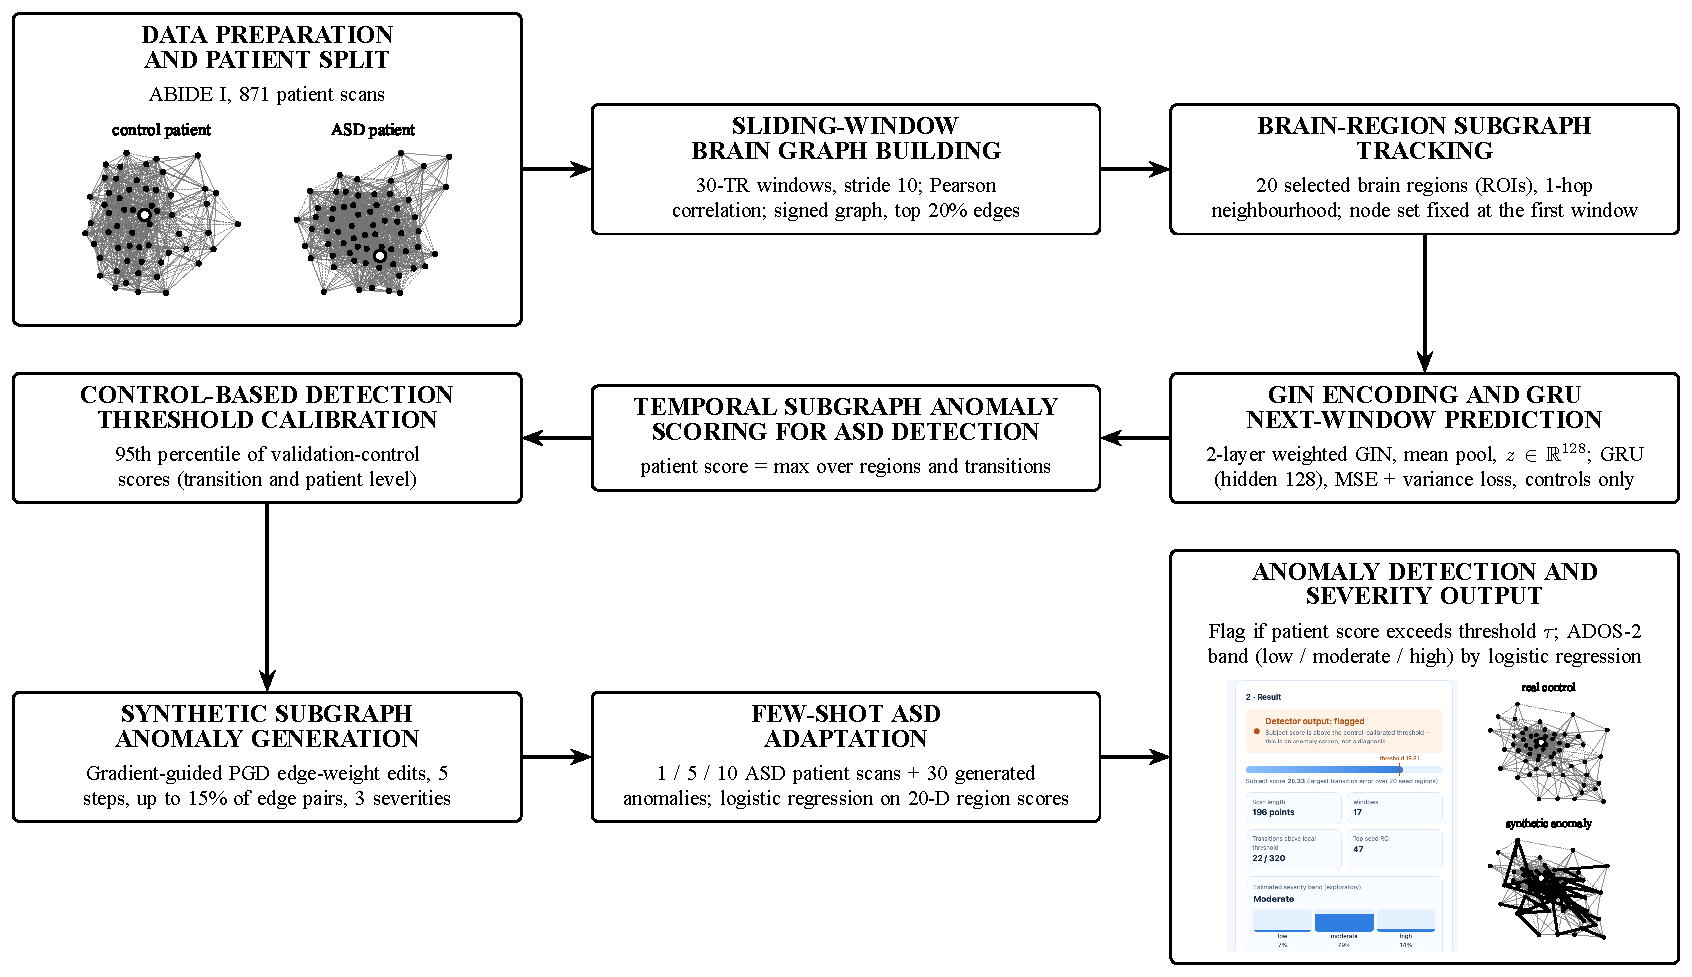
\includegraphics[width=\textwidth]{figures/fig_flow_compact.pdf}
\caption{End-to-end pipeline, read left to right on rows 1 and 3 and right to left on row 2. Test scans are used only at the final detection step.}
\label{fig:pipeline}
\end{figure}

\smallskip
The whole system as nine steps in one continuous flow, read left to right on rows 1 and 3 and right to left on row 2, with the key technical settings inside each box: 30-TR windows with top-20% signed graphs, 20 selected brain regions tracked as subgraphs, a 2-layer GIN with a GRU, the prediction-error score, a 95th-percentile threshold from control scans, gradient-guided synthetic edits, few-shot logistic regression and ADOS-based severity bands. Test scans are used only at the final detection step.

\bigskip
\clearpage
\section*{Table II: Dataset and preprocessing summary}
\begin{table}[!tbp]
\caption{Dataset and preprocessing summary.}
\label{tab:data}
\centering\footnotesize
\begin{tabular}{@{}p{2.9cm}p{5.05cm}@{}}
\toprule
Item & Value \\
\midrule
Source & ABIDE I {[3]}, ROI time series \\
Subjects & 871 (403 ASD, 468 control), 20 sites \\
ROIs; scan length & 360; 78--316 TR (5--29 windows) \\
Atlas, preprocessing & Glasser 360; CPAC, band-pass, GSR, QC-checked (released series) \\
Split (subject level) & 609 / 131 / 131; train 328 C + 281 A; val 70 C + 61 A; test 70 C + 61 A \\
Window; stride & 30 TR; 10 TR \\
Connectivity; edges & Pearson, signed; top 20\% by $|r|$ (12,924 pairs) \\
Seeds; neighbourhood & 20 ROIs; $k{=}1$, stable (window 1) \\
Subgraph size & mean 71.1 nodes; mean 783 edges/window \\
Scoring units & 6,560 train and 1,400 val sequences \\
\bottomrule
\end{tabular}
\end{table}

\smallskip
Lists the facts about the data the experiments rely on: the ABIDE I cohort (871 subjects, 403 ASD and 468 controls, 20 sites), 360 regions of interest, scan lengths, the 609/131/131 subject-level split, window and stride settings, how connectivity edges are kept, and the size of the subgraphs. It also states plainly that the brain atlas and preprocessing pipeline are not recorded in the project files.

\bigskip
\section*{Table III: Experimental configuration}
\begin{table}[!tbp]
\caption{Experimental configuration.}
\label{tab:config}
\centering\footnotesize
\begin{tabular}{@{}p{2.1cm}p{5.85cm}@{}}
\toprule
Component & Setting \\
\midrule
GIN & 2 layers, hidden 64, $D{=}128$, constant input 1.0, trainable $\epsilon$, ReLU after each layer, mean pool \\
GRU & 1 layer, hidden 128, linear read-out \\
Training & Adam, lr $10^{-3}$, no weight decay, batch 16 sequences, 5 epochs, $\lambda{=}0.5$ \\
Thresholds & $P_{95}$ of validation controls (transition, subject) \\
Generator & $\rho_e{=}0.15$, $\delta_{\max}{=}0.6$, $Q{=}5$, clip $[-1,1]$, $\alpha\in\{.25,.55,.9\}$; 60 base subjects $\times$ 20 seeds $\times$ 3 $\alpha$ $\times$ 2 methods \\
Few-shot head & Logistic regression, $C{=}1$, balanced; $K\in\{1,5,10\}$; 5 draws; 30 generated \\
Hardware & Apple-silicon laptop GPU (PyTorch MPS); chip model not logged for the original runs \\
Software & Python 3.13, PyTorch 2.14, PyG 2.8 (environment used for this paper's analyses) \\
\bottomrule
\end{tabular}
\end{table}

\smallskip
A reference sheet of every setting needed to reproduce the runs: the two-layer graph encoder (GIN), the recurrent predictor (GRU), training settings (Adam, 5 epochs), how the thresholds are set, the anomaly generator's parameters, the few-shot classifier, and the hardware and software used. Hyperparameters were fixed in advance, not searched.

\bigskip
\clearpage
\section*{Figure 2: Training curves}
\begin{figure}[!tbp]
\centering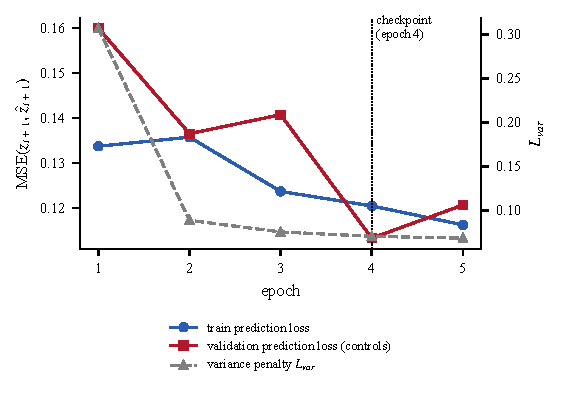
\includegraphics[width=\columnwidth]{figures/fig_training.pdf}
\caption{Training curves (5 epochs, train-control subjects). Source: \texttt{training\_report.json}.}
\label{fig:training}
\end{figure}

\smallskip
Shows the prediction error on training controls (blue) and on held-out validation controls (red) over the five training epochs, plus the variance penalty (grey dashed) that stops the embeddings from collapsing to a constant. The validation loss is lowest at epoch 4 (0.113), which is the checkpoint used. It confirms training was stable, not that the model detects ASD.

\bigskip
\section*{Figure 3: Detector test results}
\begin{figure}[!tp]
\centering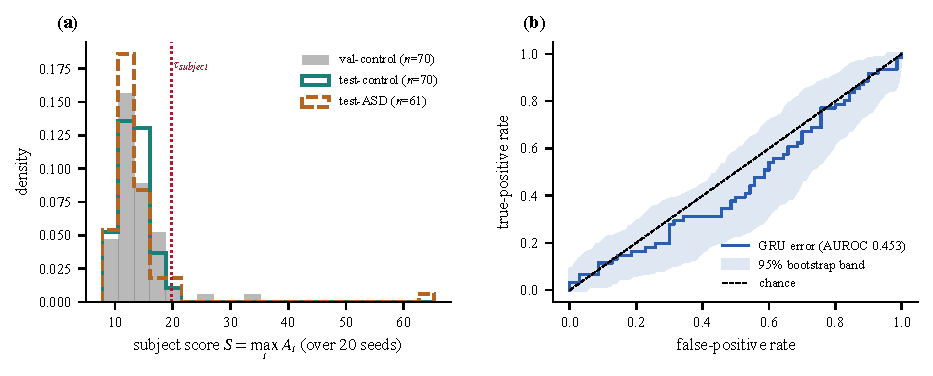
\includegraphics[width=\textwidth]{figures/fig_phase1.pdf}
\caption{Detector test results. (a) Subject scores (maximum over 20 seeds and transitions) for validation controls, test controls and test ASD subjects, with $\tau_{subject}$ (19.81). (b) ROC curve on the 131 test subjects with a 95\% bootstrap band.}
\label{fig:phase1}
\end{figure}

\smallskip
Panel (a) plots the subject-level anomaly scores of validation controls, test controls and test ASD subjects, with the decision threshold at 19.81; the three distributions overlap almost completely. Panel (b) is the ROC curve on the 131 test subjects with a 95\% bootstrap band; it hugs the chance diagonal (AUROC 0.453, CI 0.353--0.552). Together they show that the detector does not separate ASD from control subjects.

\bigskip
\section*{Figure 4: Transition scores over time for two subjects}
\begin{figure}[!tbp]
\centering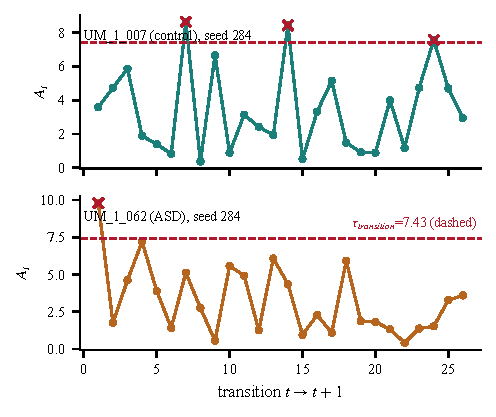
\includegraphics[width=\columnwidth]{figures/fig_timeline.pdf}
\caption{Transition scores $A_t$ for seed ROI 284 of two real test subjects (one control, one ASD) with $\tau_{transition}$ (dashed) and exceedances (crosses). The two subjects are shown for illustration only and are not representative of group differences.}
\label{fig:timeline}
\end{figure}

\smallskip
Each point is the anomaly score for one window-to-window transition of a single seed region (ROI 284) for one control subject (top) and one ASD subject (bottom). The red dashed line is the transition threshold (7.43) and crosses mark the transitions above it. It illustrates how flagged moments (the localization records) arise; the two subjects are examples only and say nothing about group differences.

\bigskip
\clearpage
\section*{Table IV: Scoring-function comparison on the test set}
\begin{table}[!tp]
\caption{Scoring-function comparison on the 131 test subjects (frozen encoder; subject score = max over seeds and transitions; threshold = $P_{95}$ of validation-control scores). AUROC with 95\% bootstrap CI and permutation $p$ against 0.5. Prevalence 0.466. Last column: AUROC when the mean over transitions replaces the maximum.}
\label{tab:scoring}
\centering\footnotesize
\resizebox{\linewidth}{!}{\begin{tabular}{@{}lcccccccc@{}}
\toprule
Scoring function & AUROC [95\% CI] & $p$ & AUPRC & Prec. & Rec. & F1 & Flagged & AUROC (mean) \\
\midrule
Static subgraph (distance to control centroid) & 0.452 [0.356, 0.553] & 0.34 & 0.489 & 0.556 & 0.082 & 0.143 & 9 & 0.455 \\
Temporal, no learned dynamics (persistence) & 0.485 [0.380, 0.582] & 0.78 & 0.484 & 0.500 & 0.033 & 0.062 & 4 & 0.508 \\
Temporal, GRU prediction error (ours) & 0.453 [0.353, 0.552] & 0.35 & 0.467 & 0.500 & 0.033 & 0.062 & 4 & 0.471 \\

Whole-graph static / temporal & \multicolumn{8}{c}{not evaluated (no whole-graph encoder was trained)} \\
\bottomrule
\end{tabular}}
\end{table}

\smallskip
Compares three ways of scoring the same frozen encoder's output: static distance from the control average, persistence (change from the previous window) and the GRU's prediction error. For each: AUROC with a 95\% bootstrap interval and permutation p-value, AUPRC, precision, recall, F1 and number of subjects flagged. All three sit near chance (AUROC 0.45--0.49, intervals overlapping), so temporal modelling gives no measurable benefit here.

\bigskip
\section*{Figure 5: Anomaly generation}
\begin{figure}[!tp]
\centering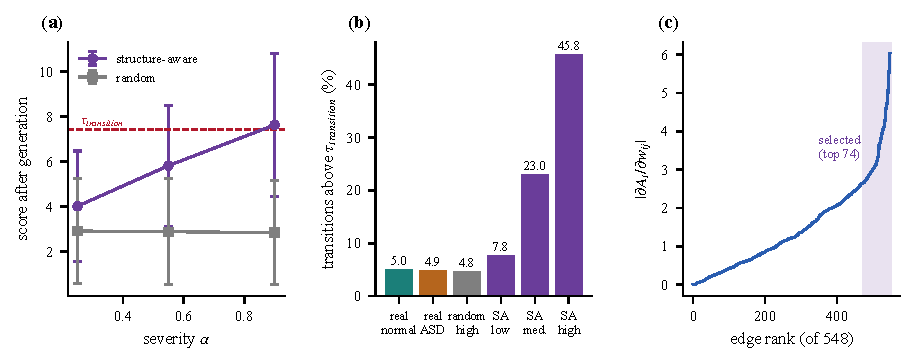
\includegraphics[width=\textwidth]{figures/fig_phase2.pdf}
\caption{Anomaly generation. (a) Score after generation vs.\ severity (mean $\pm$ SD over 1,200 records per point). (b) Fraction of transitions above $\tau_{transition}$ (SA = structure-aware). (c) Sorted gradient sensitivity for one real record (KKI\_002, seed 1) with the selected 74 of 548 edge pairs.}
\label{fig:phase2}
\end{figure}

\smallskip
(a) The model's anomaly score after editing connection weights, against edit severity: guided (structure-aware) edits raise the score steadily (about 4.0 to 7.6) while random edits do not. (b) Share of transitions above the threshold: 45.8\% for guided high-severity edits versus 4.8\% for random edits and about 5\% for real data. (c) For one example, the edges ranked by gradient sensitivity, with the 74 of 548 edge pairs chosen for editing. The effect is expected by construction because the same model guides and scores the edits.

\bigskip
\section*{Table V: Few-shot comparison on the test set}
\begin{table}[!tp]
\caption{Few-shot comparison on the 131 test subjects (mean $\pm$ SD over five support-set draws, shared test set). ``Flag'' is the mean fraction of test subjects flagged; $F1_{chance}$ is the F1 of a prevalence-matched random classifier flagging the same fraction. n/a: not derivable (precision or recall is zero in some draws).}
\label{tab:fewshot}
\centering\footnotesize
\setlength{\tabcolsep}{3pt}
\resizebox{\linewidth}{!}{\begin{tabular}{@{}clccccccc@{}}
\toprule
$k$ & Condition & Precision & Recall & F1 & AUROC & AUPRC & Flag & $F1_{chance}$ \\
\midrule
\multirow{3}{*}{1} & Few-shot only & 0.200$\pm$0.40 & 0.003$\pm$0.01 & 0.006$\pm$0.01 & 0.516$\pm$0.06 & 0.489$\pm$0.05 & n/a & n/a \\
 & + structure-aware & 0.443$\pm$0.05 & 0.344$\pm$0.04 & 0.387$\pm$0.04 & 0.497$\pm$0.03 & 0.470$\pm$0.05 & 0.36 & 0.41 \\
 & + random & 0.473$\pm$0.04 & 0.357$\pm$0.09 & 0.403$\pm$0.07 & 0.506$\pm$0.04 & 0.487$\pm$0.03 & 0.35 & 0.40 \\
\midrule
\multirow{3}{*}{5} & Few-shot only & 0.430$\pm$0.13 & 0.092$\pm$0.04 & 0.149$\pm$0.07 & 0.485$\pm$0.02 & 0.466$\pm$0.02 & 0.10 & 0.16 \\
 & + structure-aware & 0.447$\pm$0.02 & 0.348$\pm$0.04 & 0.390$\pm$0.03 & 0.486$\pm$0.03 & 0.474$\pm$0.04 & 0.36 & 0.41 \\
 & + random & 0.451$\pm$0.03 & 0.361$\pm$0.06 & 0.399$\pm$0.05 & 0.502$\pm$0.02 & 0.483$\pm$0.02 & 0.37 & 0.41 \\
\midrule
\multirow{3}{*}{10} & Few-shot only & 0.433$\pm$0.07 & 0.249$\pm$0.09 & 0.311$\pm$0.09 & 0.524$\pm$0.05 & 0.486$\pm$0.03 & 0.26 & 0.33 \\
 & + structure-aware & 0.445$\pm$0.05 & 0.367$\pm$0.05 & 0.402$\pm$0.05 & 0.501$\pm$0.05 & 0.481$\pm$0.05 & 0.38 & 0.42 \\
 & + random & 0.474$\pm$0.03 & 0.400$\pm$0.06 & 0.431$\pm$0.04 & 0.515$\pm$0.05 & 0.473$\pm$0.03 & 0.39 & 0.42 \\
\bottomrule

\end{tabular}}
\end{table}

\smallskip
Results for 1, 5 and 10 real ASD examples under three conditions: few-shot only, plus 30 structure-aware generated anomalies, plus 30 random ones (mean and standard deviation over five draws). Precision, recall, F1, AUROC and AUPRC are shown, together with the fraction of subjects flagged and the F1 a random classifier would get at that flag rate. Adding generated anomalies raises F1, but AUROC stays near 0.50 and F1 is close to the chance level.

\bigskip
\clearpage
\section*{Figure 6: Few-shot results}
\begin{figure}[!tp]
\centering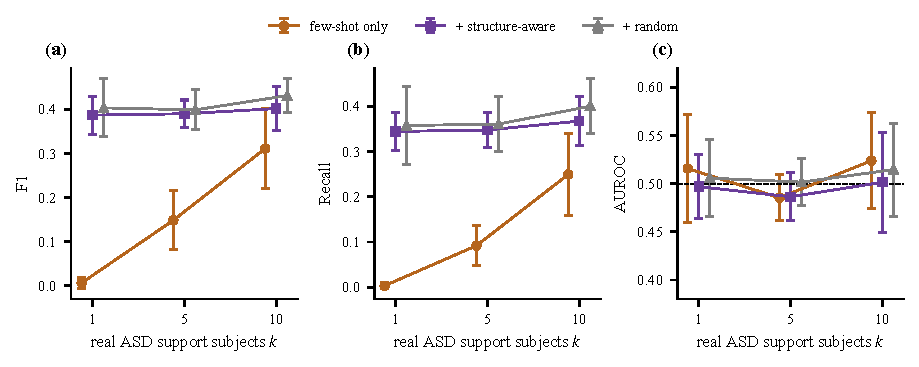
\includegraphics[width=\textwidth]{figures/fig_phase3.pdf}
\caption{Few-shot results (mean $\pm$ SD over five support draws) for (a) F1, (b) recall and (c) AUROC; the dashed line marks chance AUROC.}
\label{fig:phase3}
\end{figure}

\smallskip
The same few-shot results as a graph: F1 (a), recall (b) and AUROC (c) against the number of real ASD examples, for the three conditions with error bars. F1 and recall jump when generated anomalies are added, but AUROC stays on the dashed chance line (0.5) in every condition. This indicates the classifier flags more subjects rather than ranking ASD subjects better.

\bigskip
\section*{Table VI: Severity-band estimation (exploratory)}
\begin{table}[!tbp]
\caption{Severity-band estimation (3 classes: low, moderate, high). Majority-class accuracy is the accuracy of always predicting the most common training band; uniform chance is 0.333.}
\label{tab:severity}
\centering\footnotesize
\begin{tabular}{@{}lcccc@{}}
\toprule
Evaluation & $n$ & Accuracy & Macro-F1 & Majority \\
\midrule
Held-out (val.\ + test ASD) & 60 & 0.433 & 0.395 & 0.550 \\
5-fold CV $\times$10 (all) & 193 & 0.391$\pm$0.066 & 0.372 & 0.430 \\
\bottomrule
\end{tabular}
\end{table}

\smallskip
Tests whether the detector's scores can estimate ADOS-2 based severity bands (low, moderate, high) for ASD subjects. Accuracy and macro-F1 are given for a held-out set (60 subjects) and for repeated cross-validation (193 subjects), next to the accuracy of always guessing the most common band. The model is below that simple rule, so the scores carry no usable severity information here.

\bigskip
\section*{Table VII: Component ablation and coverage}
\begin{table}[!tbp]
\caption{Component ablation and coverage.}
\label{tab:ablation}
\centering\footnotesize
\setlength{\tabcolsep}{3pt}
\begin{tabular}{@{}p{2.25cm}p{3.6cm}p{1.7cm}@{}}
\toprule
Component & Comparison and outcome & Status \\
\midrule
Temporal model & GRU vs.\ persistence vs.\ static: AUROC 0.453 / 0.485 / 0.452, CIs overlap & evaluated \\
Subgraph localization & vs.\ whole-graph scoring & not evaluated \\
GIN encoder & alternative encoders & not evaluated \\
Variance term & $\lambda{=}0$ & not evaluated \\
Generated anomalies & F1 up, AUROC unchanged; $F1\approx F1_{chance}$ & evaluated \\
Structure-aware vs.\ random & Generation: 45.8\% vs.\ 4.8\%; few-shot: no gain & evaluated \\
Recurrence & ASD 0.498 vs.\ control 0.488 flagged seeds & evaluated \\
Severity estimation & Accuracy 0.433 vs.\ majority 0.550 & evaluated \\
Support-weighted score & $A(1{+}\lambda C)$ & not implemented \\
\bottomrule
\end{tabular}
\end{table}

\smallskip
Summarises which parts of the method were actually tested against an alternative and what came out: temporal versus static scoring, generated anomalies, structure-aware versus random, and recurrence were evaluated; subgraph versus whole-graph scoring, alternative encoders, the variance term and a support-weighted score were not. It keeps the paper honest about what is, and is not, supported by evidence.

\bigskip
\section*{Table VIII: Computational cost}
\begin{table}[!tbp]
\caption{Computational cost (Apple-silicon laptop; GPU via PyTorch MPS except cache build on CPU).}
\label{tab:cost}
\centering\footnotesize
\begin{tabular}{@{}p{4.1cm}p{3.7cm}@{}}
\toprule
Stage & Measured \\
\midrule
Cache 20 seeds, 871 subjects (CPU) & 112 s \\
Joint training (5 epochs) & 299.7 s \\
Detector evaluation and localization & 27 s \\
Generate 7,200 records & 79 s \\
45 few-shot fits + scoring & 86 s \\
All-360-seed extraction & 71.5 s/subject; 98.5 MB peak \\
\bottomrule
\end{tabular}
\end{table}

\smallskip
Measured run times on an Apple-silicon laptop: building the subgraph cache (112 s), training (299.7 s), the detector evaluation (27 s), generating 7,200 anomaly records (79 s), the 45 few-shot fits (86 s), and the cost of extracting all 360 seed subgraphs per subject. It shows the whole pipeline is cheap enough to run on a laptop.

\bigskip
\end{document}
